\documentclass{article}
\usepackage{url}
\usepackage{mathtools}
\usepackage{amsmath}
\usepackage{listings}
\usepackage{graphicx}
\usepackage[margin=1in]{geometry}
\usepackage{float}
\floatstyle{boxed}
\restylefloat{figure}
\lstset{breaklines=true}
\begin{document}

\title{CS595 Intro to Web Science, Assignment \#2}
\author{Valentina Neblitt-Jones}
\date{September 26, 2013}
\maketitle

\section{Link Extraction from Twitter}
\textbf {Write a Python program that extracts 1000 unique links from Twitter. You might want to take a look at: \url{http://thomassileo.com/blog/2013/01/25/using-twitter-rest-api-v1-dot-1-with-python/}. But there are many other similar resources available on the web. Note that only Twitter API 1.1 is currently available; version 1 code will no longer work. Also note that you need to verify that the final target URI (i.e., the one that responds with a 200) is unique. You could have different shortened URIs for www.cnn.com. You might want to use the search feature to find URIs, or you can pull them from the feed of someone famous (e.g., Tim O'Reilly). Hold on to this collection. We'll use it later through the semester.}


\subsection*{The Files}
Files Used to Complete Q1

\begin{enumerate}
\item TwitterLink.py - Gathering tweets from 27 users
\item tweetlink.txt - File created by TwitterLink.py - contains URIs retrieved from tweet
\item UnpackURIs.py - Unshorten links from tweets
\item unpackedURLs.txt - File created by UnpackURIs.py - contains full URIs
\item DedupeURIs.py - Remove duplicate URIs
\item uniqueURIs.txt - File created by DedupeURIs - contains unique URIs
\end{enumerate}

\subsection*{Tweeters}
I used 27 tweeters. I could have used less by continuing to loop through some of the more prolific tweeters' timelines, but I thought more tweeters would provide a better variety of links and reduce the risk of getting duplicate links.

\begin{itemize}
\item Michael Moore
\item Rachel Maddow
\item New York Times
\item Sesame Street
\item The Daily Show
\item Washington Post
\item Barack Obama
\item Cory Booker
\item Joel Spolsky
\item Governor Christie
\item Planned Parenthood
\item National Zoo
\item United Nations
\item Washington City Paper
\item Entertainment Weekly
\item TMZ
\item NPR
\item Virginia Tech News
\item New York Public Library
\item Library of Congress
\item Chicago Sun Times
\item Chicago Tribune
\item USA.gov
\item Harvard University
\item NFL
\item NPR News
\item Neil deGrasse Tyson
\end{itemize}

\subsection*{The Code}

I divided this part of the assignment into three Python programs - one to gather links from tweets, another to unshorten the links, and a third to remove duplicates. First I modified the file provided by Thomas Sileo as was suggested in the assignment. The segment below shows one example of how I gathered 200 tweets from a tweeter. It goes through the maximum number of tweets allowed at one time, looks for a link and captures it and writes it to a file called tweetlink.txt. I captured 3553 links total. An portion of the output can be seen in Figure \ref{shorturls}.

\begin{lstlisting}
	f = open(`tweetlink.txt', `w')

        print(``'')
        print``Joel Spolsky Tweet'')
        print(``'')
        screen_name9 = ``spolsky''
        count = ``200''
        uri = ``https://api.twitter.com/1.1/statuses/user_timeline.json?'' + ``screen_name='' + screen_name9 + ``&count='' + count
        r = requests.get(uri, auth=oauth)
        l = r.json()
        for tweet in l:
            try:
                f.write(tweet[`entities'][`urls'][0][`expanded_url'])
                f.write(``\n'')
            except UnicodeEncodeError:
                pass
            except IndexError:
                pass
\end{lstlisting}

\begin{figure}[H]
\centering
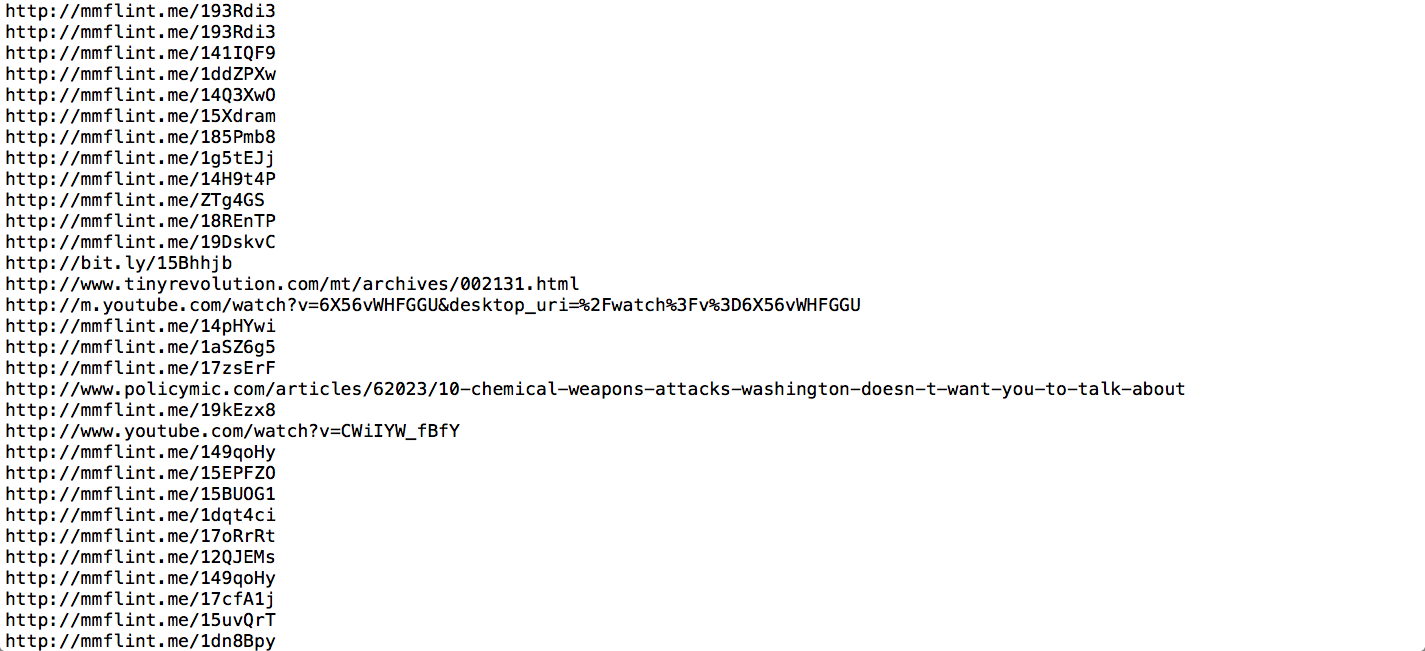
\includegraphics[scale=0.25]{q1/shortened}
\caption{Output from TwitterLinks.py}
\label{shorturls}
\end{figure}

Next I tackled unshortening the links. The program used tweetlinks.txt as an input file and wrote out to unpackedURLs.txt. There were some errors in my first drafts of the program because I had not handled the errors and could not tell how things were progressing. Some print statements let me know that I was throwing out some of them since they did not resolve themselves and the flush allowed results to be written to the file before the whole program completed. I had 2959 links left after this process. An portion of the output can be seen in Figure \ref{unshorturls}.

\begin{lstlisting}
f = open(`tweetlink.txt', `r')
s = open(`unpackedURLs.txt', `w')

for line in f:
    print(line)
    try:
        a = urllib.request.urlopen(line)
        good = a.geturl()
        s.write(good)
        print(`Kept ' + line + ` as ' + good)
        s.write(`\n')
        s.flush()
        os.fsync(s.fileno())
    except:
        print(`Throwing out ' + line)
        pass

f.close()
s.close()
\end{lstlisting}

\begin{figure}[H]
\centering
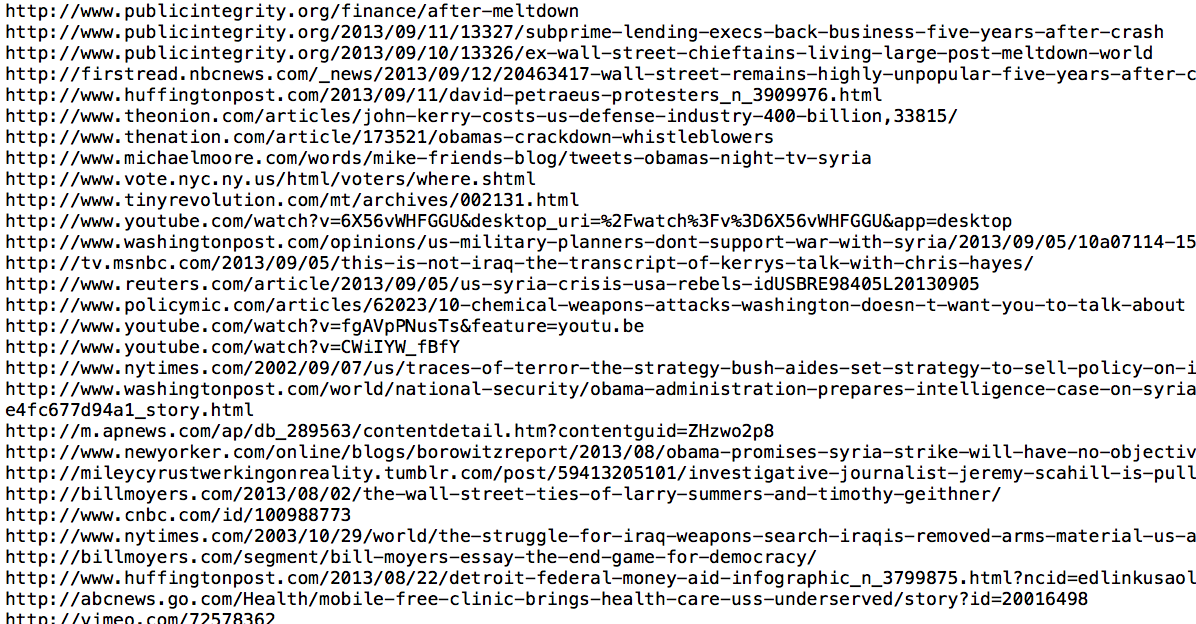
\includegraphics[scale=0.25]{q1/unshortened}
\caption{Output from UnpackURIs.py}
\label{unshorturls}
\end{figure}

The last part of this was to make sure the links were unique. I consulted Stack Overflow for converting between a set and a list in Python. There were 2454 links remaining after this process.

\begin{lstlisting}
f = open(`unpackedURLs.txt', `r')
s = open(`uniqueURIs.txt', `w')

#read file in as a list
#Python documentation http://docs.python.org/3.3/tutorial/inputoutput.html

urilist = f.readlines()
print(len(urilist)) #test of number of URIs before

#convert list to a set
#from Stack Overflow http://stackoverflow.com/questions/6593979/how-to-convert-a-set-to-a-list-in-python

uriset = set(urilist)

print(len(uriset)) #test of number of URIs after

#write set contents to a file

for uri in uriset:
    s.write(uri)
\end{lstlisting}

\newpage

\section{TimeMaps Exercise}
\textbf{Download the TimeMaps for each of the target URIs. We'll use the ODU Memento Aggregator, so for example:}

\textbf{URI-R = \url{http://www.cs.odu.edu}}

\textbf{URI-T = \url{http://mementoproxy.cs.odu.edu/aggr/timemap/link/http://www.cs.odu.edu/}}

\textbf{Create a histogram of URIs vs. number of Mementos (as computed from the TimeMaps). For example, 100 URIs with 0 Mementos, 300 URIs with 1 Memento, 400 URIs with 2 Mementos, etc.}

\subsection*{The Files}
Files Used to Complete Q2

\begin{enumerate}
\item uniqueURIs2.txt - Copy of file created by DedupeURIs - contains unique URIs
\item GetTimemaps.py - Loops through unique URIs to aggregate and count the number of mementos for each
\item timeMapResults.txt - Output of the URIs and number of mementos found for each
\item TimeMapAnalysis.xslx - Excel workbook that has the raw data, processed data and the histogram (Figure \ref{urivmementos})
\end{enumerate}

\subsection*{The Code}
Even though I only had one program for this part of the assignment, it took quite a while to completely execute the program. From Figure \ref{aggtime}, you can see that it took approximately 8 hours to run. Outputting to the screen and writing to the file was even more important with this one. In the first attempt, I let it run overnight and could not tell if it had finished in the morning as my computer likes to take naps. I had to run it again, but added the same type of safeguards from the unshortening exercise in Q1.

\begin{figure}[H]
\centering
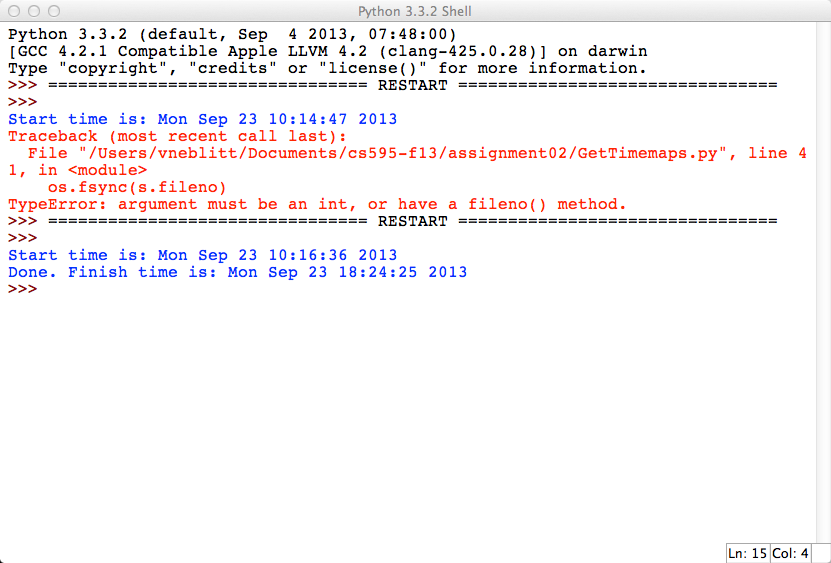
\includegraphics[scale=0.50]{q2/MementoAggregatorRunTime}
\caption{Start and Finish Time for Memento Aggregator}
\label{aggtime}
\end{figure}

I consulted Python's documentation \url{http://docs.python.org/3/howto/regex.html} about using regular expressions since the items I needed to count contained the word ``memento.'' I had three failed attempts to develop the proper expression - one returned errors, another returned 0 and a third returned almost the correct answer (counted everything but the first and last memento). I shortened the input file and renamed it since it was warned on the email list that this would take a long time and going through 2454 links would far too long to complete. My code runs through the input file and prepend the http://mementoproxy.cs.odu.edu/aggr/timemap/link/ before attempting to open it.

\begin{lstlisting}
pattern = re.compile(`rel=``[(first | last)]*memento''')

f = open(`uniqueURIs2.txt', `r')
s = open(`timeMapResults.txt', `w')

uriprepend = `http://mementoproxy.cs.odu.edu/aggr/timemap/link/'

for line in f:
    #print(uriprepend + line)
    try:
        a = uriprepend + line
        r = urllib.request.urlopen(a)
        #print(`TimeMaps found for ' + line)
        timemap = r.read()
        c = pattern.findall(timemap.decode(`utf-8'))
        #print(line.rstrip() + " produces " + str(len(c)) + `` timemaps'')
        s.write(line.rstrip() + ``, '' + str(len(c)) + ``\n'')
        s.flush()
        os.fsync(s.fileno())
    except urllib.error.HTTPError:
        #print(`No TimeMaps found for ' + line)
        s.write(line.rstrip() + ``, 0\n'')
        s.flush()
        os.fsync(s.fileno())
        pass

f.close()
s.close()
\end{lstlisting}

The second part of the question asked for a histogram. During my first attempt to produce this, it was evident that I did not understand what a histogram was and needed to understand a rudimentary example first. I found a short video online \url{http://www.youtube.com/watch?v=KCH_ZDygrm4} that explained the fundamentals. I then followed an example for Excel 2007 to determine how it would produce one \url{http://support.microsoft.com/kb/214269}. The output in Figure \ref{urivmementos} shows that 837 of my 1002 URIs have zero mementos. Then the number of URIs with one or more mementos decreases sharply.

\begin{figure}[H]
\centering
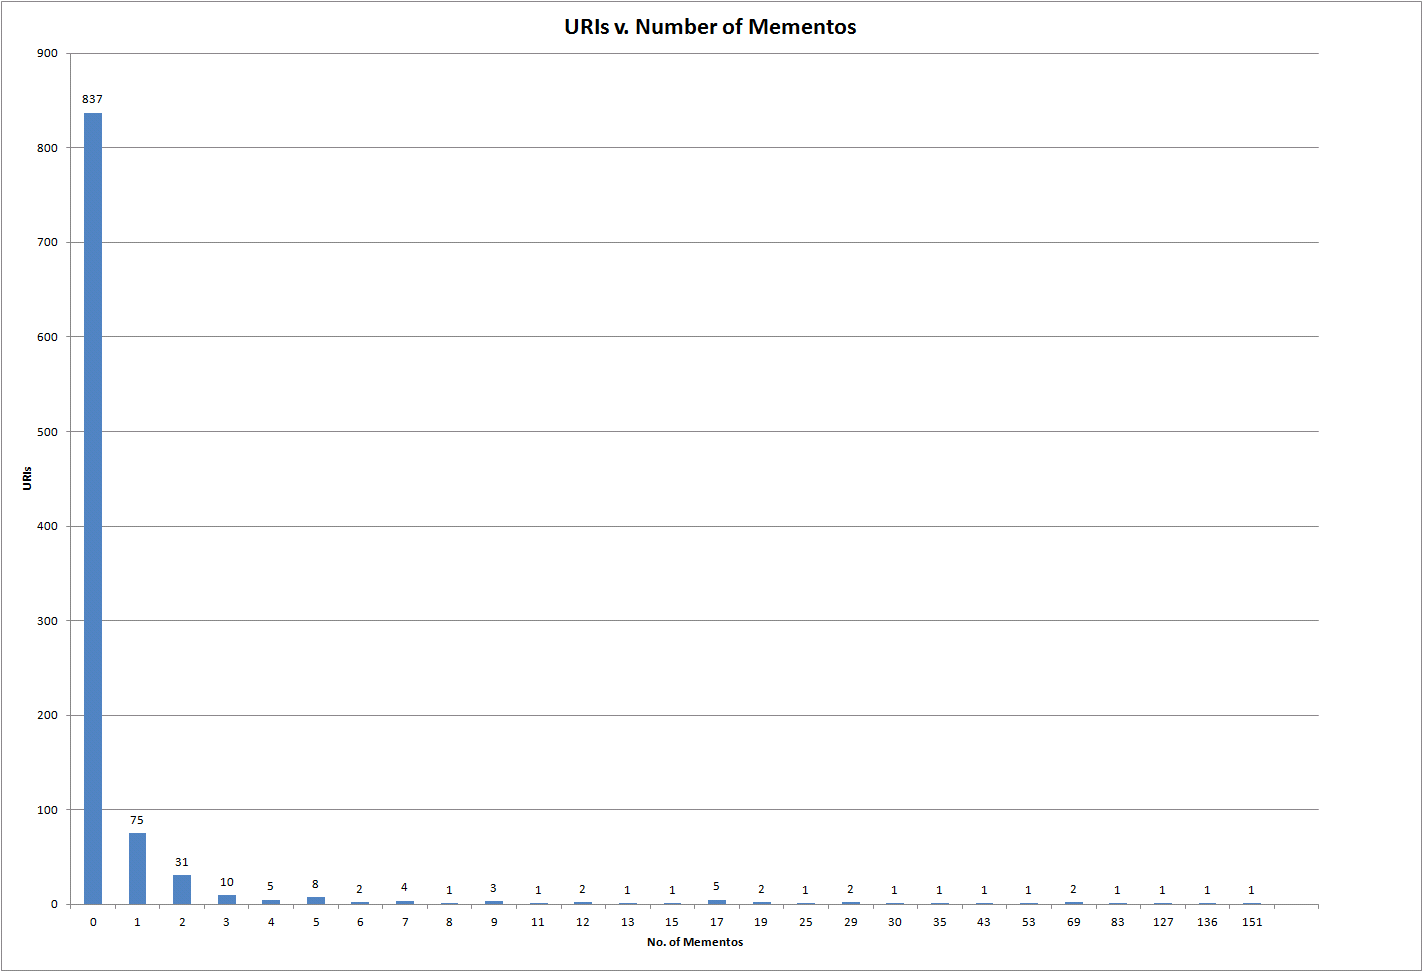
\includegraphics[scale=0.25]{q2/histogram}
\caption{URIs vs. Number of Mementos}
\label{urivmementos}
\end{figure}

\newpage

%\begin{lstlisting}
%\end{lstlisting}

\section{Carbon Date Exercise}
\textbf{Estimate the age of each of the 1000 URIs using the ``Carbon Date'' tool: \url{http://ws-dl.blogspot.com/2013/04/2013-04-19-carbon-dating-web.html}. Note you'll have to download and install; don't try to use the web service. For URIs that have \textgreater  0 Mementos and an estimated date, create a graph with age (in days) on one axis and number of Mementos on the other.}

\subsection*{The Files}
Files Used to Complete Q3

Since this part of the assignment relied on a program created by Hany SalahEldeen and it was written for Python 2.6, I switched from using Python 3.3.2 to using Python 2.7.5.

\begin{enumerate}
\item timeMapResults2.txt - Copy of the file created by GetTimeMaps.py. Used UNIX shell command to create five smaller files of 200 each to prepare for simultaneously processing.
	\begin{verbatim}
	split -l 200 timeMapResults2.txt
	\end{verbatim}
	\begin{enumerate}
		\item tmaa
		\item tmab
		\item tmac
		\item tmad
		\item tmae
	\end{enumerate}
\item carbonDatingLocal.py - Modified Hany's code take three arguments (script name, input file name, output file name) and produce five output files.
	\begin{verbatim}
	/usr/local/bin/python carbonDatingLocal.py tmaa tm01
	\end{verbatim}
	\begin{enumerate}
		\item tm01
		\item tm02
		\item tm03
		\item tm04
		\item tm05
	\end{enumerate}
\item carbonDateResults.txt - concatenation of the five smaller files into a single file
\begin{verbatim}
cat tm01 tm02 tm03 tm04 tm05 > carbonDateResults.txt
\end{verbatim}
\item getURIAge.py - Converts date output in carbonDateResults.txt to a date time object and then calculates age in days
\item URIAgeResultsGraph.xslx - Excel workbook that has the data and the graph (Figure \ref{agevmementos})
\end{enumerate}

\subsection*{The Code}
Even though I was running five lists of 200 each at the same time, this did not finish even after 20 hours. Two of the five processes finished (reached 200). One got really close (reached 193). Another got halfway there (reached 100). The saddest one only reach 9. It was stuck at the 9th link for 12 hours. I noticed the ones that got stuck or took a long time tended to be YouTube videos and were getting stuck on the Backlinks checking part. So I had to end it and only managed to get 707 carbon dates. Figure \ref{hangup} shows one of the ``hangups'' on a YouTube video just after Google finished and Backlinks was processing.

\begin{figure}[H]
\centering
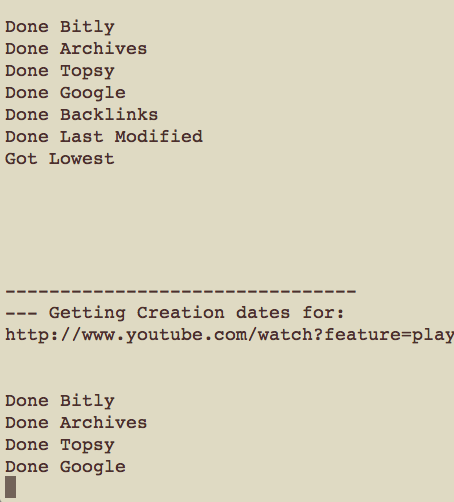
\includegraphics[scale=0.50]{q3/carbonDateRunning}
\caption{Example of carbonDatingLocal.py Running}
\label{hangup}
\end{figure}

I only returned Lowest from Hany's local program. I added the safeguards again from Q1 in order to monitor progress and capture output as it was being produced. My input file had commas separating the elements and that was a big mistake since some of my URIs had commas in them. I had to use Python's split function \url{http://stackoverflow.com/questions/14351356/python-line-split} to create a better delimiter.

\begin{lstlisting}
	return lowest
   

if(len(sys.argv)!=3):
	print ``wrong format''
else:
        start = time.localtime()
        print `Start time is: ' + time.asctime(start)
        
        inputfile = sys.argv[1]
        outputfile = sys.argv[2]
        f = open(inputfile)
        s = open(outputfile, 'w')
        for line in f:
                line = line.strip()
                (url, count) = line.split(`, ')
                cd = carbonDate(url)
                s.write(url + `\t' + count + `\t' + cd + `\n')
                s.flush()
                os.fsync(s.fileno())
        f.close()
        s.close()

\end{lstlisting}

The output of the carbon date was not suitable for calculating age of the URI so I needed to write another program (getURIage.py) to process the carbon date into age. I had to split the line again to create the three elements, then convert the carbon date to a date time object. Only then was I able to subject current date time from the processed carbon date time and reference as days.

\begin{lstlisting}
f = open('carbonDateResults.txt', `r')
s = open('URIAgeResults.txt', `w')

for line in f:
    line = line.strip()
    try:
        (url, count, cd) = line.split(`\t')
        currenttime = datetime.datetime.now()
        if cd:
            carbontime = datetime.datetime.strptime(cd, '\%Y-\%m-\%dT\%H:\%M:\%S')
            difference = currenttime - carbon time
            age = difference.days
            s.write(url + `\t' + count + `\t' + str(age) + `\n')
    except ValueError:
        pass

f.close()
s.close()

\end{lstlisting}

I used Excel again to produce the requested graph of age in days versus number of mementos.

\begin{figure}[H]
\centering
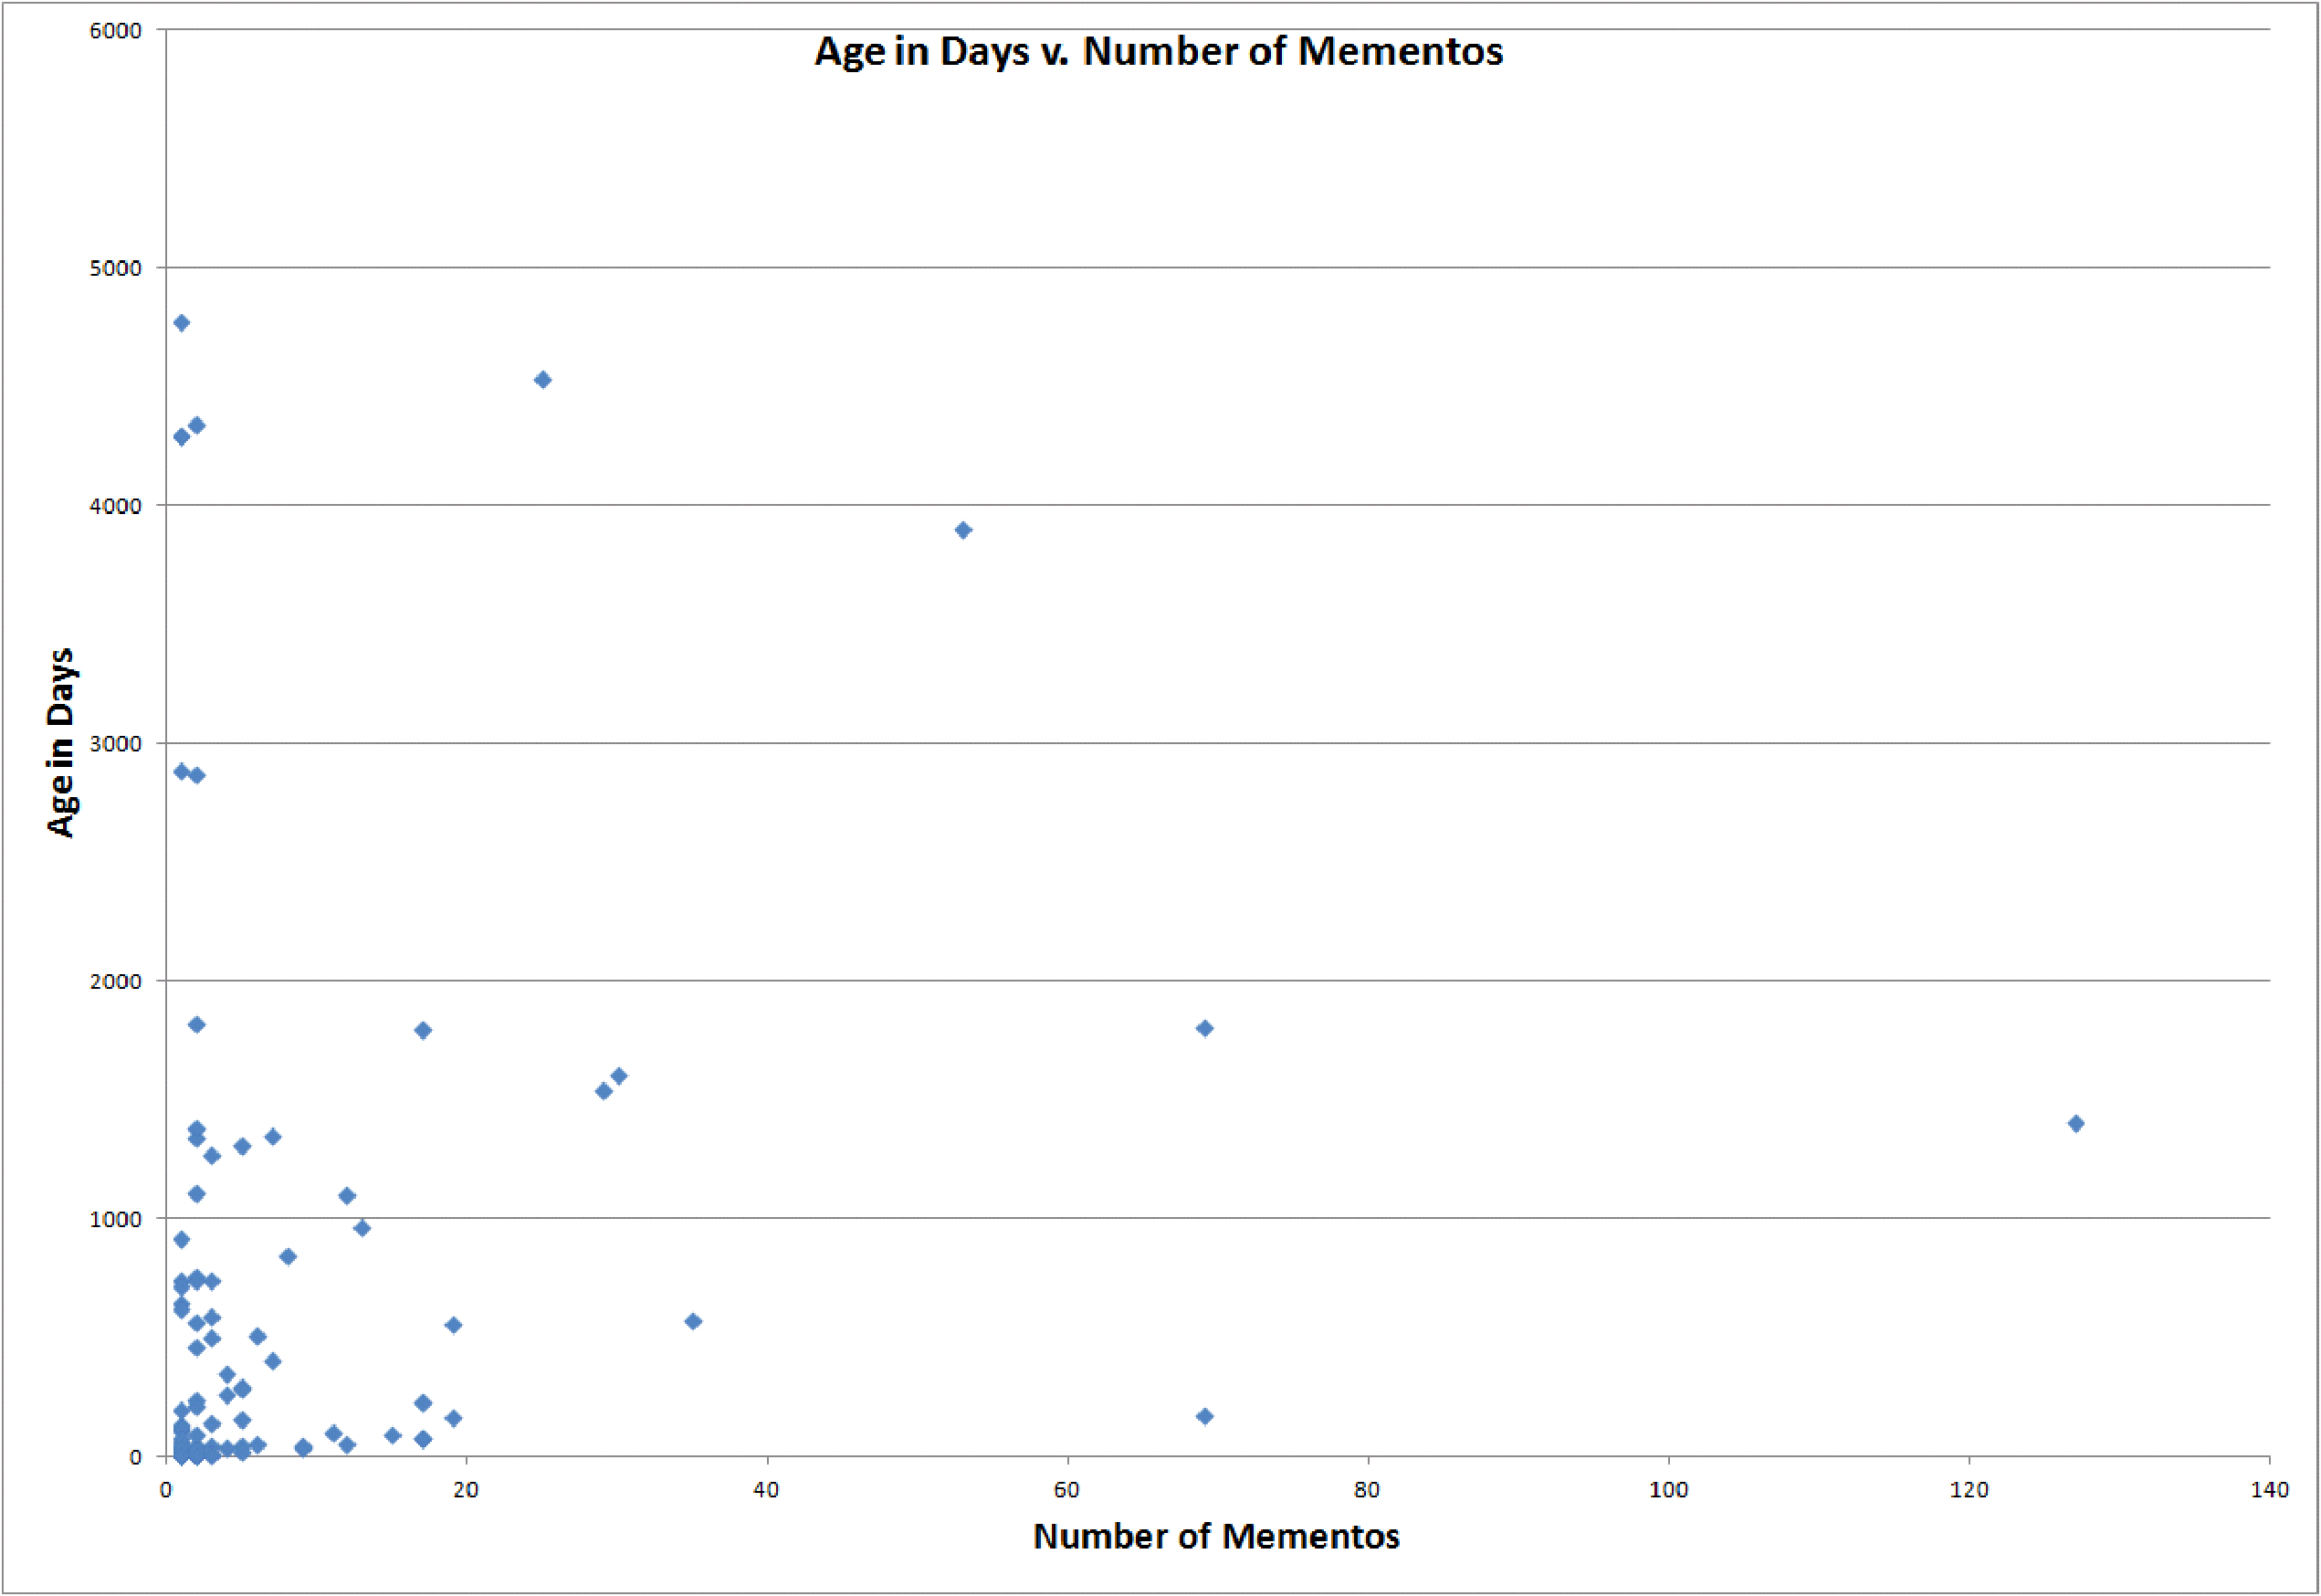
\includegraphics[scale=0.25]{q3/uriAgeGraph}
\caption{Age in Days vs. Number of Mementos}
\label{agevmementos}
\end{figure}

\end{document}